\documentclass[
  bibliography=totoc,     % Bibliography as unnumbered chapter in toc
  numbers=noenddot,       % No dot after figure/table number
  captions=tableheading,  % Correct spacing for table headings
  % titlepage=firstiscover, % Symmetrical margins on titlepage
  parskip=half,           % Hals skip instead of intend in new paragraph
  headings=normal,
  a4paper,
]{scrartcl}

% Warning, if another latex run is needed
\usepackage[aux]{rerunfilecheck}
\setcounter{tocdepth}{2}

%------------------------------------------------------------------------------
%-- Language and Type
%------------------------------------------------------------------------------
\usepackage{fontspec}
\defaultfontfeatures{Ligatures=TeX}  % -- becomes en-dash etc.

% Language: english | german
\usepackage{polyglossia}
\setdefaultlanguage{english}

% For german | english abstract and german | english titles in the toc
\setotherlanguages{english}

% Intelligent quotation marks, language and nesting sensitive
\usepackage[autostyle]{csquotes}

% Microtypographical features, makes the text look nicer on the small scale
\usepackage{microtype}

%------------------------------------------------------------------------------
%-- Math
%------------------------------------------------------------------------------
\usepackage{amsmath}
\usepackage{amssymb}
\usepackage{mathtools}

% Enable Unicode-Math and follow the ISO-Standards for typesetting math
\usepackage[
  math-style=ISO,
  bold-style=ISO,
  sans-style=italic,
  nabla=upright,
  partial=upright,
]{unicode-math}
\setmathfont{Latin Modern Math}

\usepackage{xfrac}   % Small fracs for the text with \sfrac{}{}
\usepackage{braket}  % Good for expectation values

%------------------------------------------------------------------------------
%-- Numbers and Units
%------------------------------------------------------------------------------
\usepackage[
  locale=US,
  separate-uncertainty=true,
  per-mode=symbol-or-fraction,
  exponent-product=\cdot,
]{siunitx}
\sisetup{math-micro=\text{µ},text-micro=µ}

%------------------------------------------------------------------------------
%--Tables
%------------------------------------------------------------------------------
\usepackage{booktabs}  % Use \toprule, \midrule, \bottomrule

%------------------------------------------------------------------------------
%-- Graphics
%------------------------------------------------------------------------------
\usepackage{graphicx}
\usepackage{grffile}

%------------------------------------------------------------------------------
%-- Colors
%------------------------------------------------------------------------------
\usepackage{xcolor}
\xdefinecolor{darkgrey}{HTML}{353132}
% Nord colors: https://github.com/arcticicestudio/nord
% Polar Night (dark greys)
\xdefinecolor{nordgrey1}{HTML}{2E3440}
\xdefinecolor{nordgrey2}{HTML}{3B4252}
\xdefinecolor{nordgrey3}{HTML}{434C5E}
\xdefinecolor{nordgrey4}{HTML}{4C566A}
% Snow Storm (muted whites)
\xdefinecolor{nordwhite1}{HTML}{D8DEE9}
\xdefinecolor{nordwhite2}{HTML}{E5E9F0}
\xdefinecolor{nordwhite3}{HTML}{ECEFF4}
% Frost (cool blues/greens)
\xdefinecolor{nordbluegreen}{HTML}{8FBCBB}
\xdefinecolor{nordcyan}{HTML}{88C0D0}
\xdefinecolor{nordpaleblue}{HTML}{81A1C1}
\xdefinecolor{norddeepblue}{HTML}{5E81AC}
% Aurora (muted accent colors)
\xdefinecolor{nordred}{HTML}{BF616A}
\xdefinecolor{nordorange}{HTML}{D08770}
\xdefinecolor{nordyellow}{HTML}{EBCB8B}
\xdefinecolor{nordgreen}{HTML}{A3BE8C}
\xdefinecolor{nordviolet}{HTML}{B48EAD}

%------------------------------------------------------------------------------
%-- Floats
%------------------------------------------------------------------------------
% Allow figures to be placed in the running text by default:
\usepackage{scrhack}
\usepackage{float}
\floatplacement{figure}{htbp}
\floatplacement{table}{htbp}

\usepackage[section, below]{placeins}  % Keep figures and tables in the section

\usepackage{caption}
\usepackage{subcaption}

%------------------------------------------------------------------------------
%-- Customize list environments
%------------------------------------------------------------------------------
\usepackage{enumitem}

%------------------------------------------------------------------------------
%-- Bibliography
%------------------------------------------------------------------------------
\usepackage[
  backend=biber,    % use modern biber backend
  autolang=hyphen,  % load hyphenation rules for if language of bibentry is not
                    % german, has to be loaded with \setotherlanguages
                    % in the references.bib use langid={en} for english sources
]{biblatex}

%------------------------------------------------------------------------------
%-- Code environment and verbatim
%------------------------------------------------------------------------------
\usepackage{listings}
\lstset{basicstyle=\ttfamily}
\newcommand{\code}[1]{\lstinline|#1|}

%------------------------------------------------------------------------------
%-- Misc
%------------------------------------------------------------------------------
\usepackage[pdfusetitle,unicode,]{hyperref}
\hypersetup{
  unicode=true,
  colorlinks,
  linkcolor=black,
  citecolor=black,
  filecolor=black,
  urlcolor=norddeepblue,
}
\usepackage{bookmark}
\usepackage[shortcuts]{extdash}
\usepackage{scrlayer-scrpage}  % For custom KOMA layout modifications

%------------------------------------------------------------------------------
%-- Custom math operators
%------------------------------------------------------------------------------

\newcommand{\mperiod}{\quad\text{.}}
\newcommand{\mcomma}{\quad\text{,}}
\newcommand{\mintertext}[1]{\quad\text{#1}\quad}

\renewcommand{\d}[1]{\mathrm{d}#1}
\newcommand{\del}[1]{\partial #1}
\newcommand{\dd}[2]{\frac{\d{#1}}{\d{#2}}}
\newcommand{\deldel}[2]{\frac{\partial #1}{\partial #2}}

\DeclareMathOperator{\rect}{rect}
\DeclareMathOperator{\diag}{diag}
\DeclareMathOperator{\trace}{trace}


% \addbibresource{references.bib}


\begin{document}

\begin{titlepage}
  \centering
  {\scshape\Large Analysis Note\par}
  \vspace{1.5cm}
  {\huge\bfseries Time Dependent Point Source Stacking Search Associated with HESE Track Events\par}
  \vspace{2cm}
  {\Large Thorben Menne\par}

  \vfill

  % Bottom of the page
  \textsc{Transients Working Group}\par
  \url{https://wiki.icecube.wisc.edu/index.php/Transients_Working_Group}\par
  \vspace{0.5cm}
  \textsc{Reviewers}\par
  \begin{tabular}{rl}
    \centering
    Collaboration: & Sandro Kopper (\href{mailto:sjkopper@ua.edu}{sjkopper@ua.edu}) \\
    Working Group: & Kevin Meagher (\href{mailto:kmeagher@ulb.ac.be}{kmeagher@ulb.ac.be}) \\
  \end{tabular}\par
  \vspace{0.5cm}
  \textsc{Contact}\par
  \begin{tabular}{rl}
    \centering
    Mail: & \href{mailto:thorben.menne@tu-dortmund.de}{thorben.menne@tu-dortmund.de} \\
    Slack: & @mennthor
  \end{tabular}\par
  \vspace{2cm}
  {\Large Last edit: \today\par}
\end{titlepage}

\tableofcontents
\newpage


\section{Overview}
This analysis is searching for a stacked lower energy neutrino contribution at the HESE track event positions, which are treated as transient sources.
We test for 21 generic box time windows increasing in logarithmic time from 2 seconds to 5 days symmetrically around all sources.

For the physics motivation: IceCube couldn't find a significant point source so far despite many different analysis and efforts.
Prominent examples relevant for this is search are the \href{time integrated 7 year point source search} and the \href{HESE 6 year point source search}, both with no significant results.
But the HESE events on their own show a clear astrophysical signal and therefore should originate from some sources.
This analysis test if there is any clustering of lower energy neutrino events around the HESE locations.

The analysis method is a time dependent unbinned likelihood approach similar to the so called \enquote{GRB Likelihood}.
Key features used here are:
\begin{itemize}
  \item Background is modelled using scrambled data
  \item Using time dependent spatial background PDFs
  \item Energy PDF is estimated from data and MC with fixed index $E^{-2}$ power law
\end{itemize}

For source and test data we use:
\begin{itemize}
  \item Source dataset: 6 years HESE track events, IC79 - IC86, 2015.
  \item Test dataset: 5 years PS tracks (IC79 - IC86, 2014) + 1 year GFU (IC86, 2015)
\end{itemize}

The wiki can be found at \url{https://wiki.icecube.wisc.edu/index.php/Transient_HESE_Stacking} and contains this analysis note.



\section{Software}
The analysis scripts are in a git repository and can be found at \path{/home/tmenne/analysis/hese_transient_stacking/analysis}.
Code is enumerated in the order of script execution, if someone wants to redo all analysis steps.
The branch for this analysis is \code{original_hese} which tests the 22 original HESE track events.

The main analysis software used is made from scratch in python with a small C++ back-end for time consuming work with inspiration from \href{http://code.icecube.wisc.edu/projects/icecube/browser/IceCube/sandbox/skylab}{skylab} and \href{http://code.icecube.wisc.edu/projects/icecube/browser/IceCube/sandbox/richman/grbllh}{grbllh}.
The software repository can be found at \path{/home/tmenne/software/tdepps}.
The branch used for the analysis is \code{new_structure}.



\section{Datasets}
This analysis used HESE track events as sources and point source and GFU samples as a test dataset.

\subsection{Sources}
For source positions, the 22 HESE track events from 6 years of HESE data are tested.
The list of events can be seen at the list of \href{https://wiki.icecube.wisc.edu/index.php/Analysis_of_pre-public_alert_HESE/EHE_events#HESE
}{pre-public alert HESE events}.
For each of these events detailed \href{http://software.icecube.wisc.edu/documentation/projects/millipede/index.html}{millipede} scans exist.
The best fit positions are taken from these maps for the tested source positions by converting the best fit pixel in local coordinates to equatorial coordinates using the \href{http://software.icecube.wisc.edu/documentation/projects/astro/index.html}{astro} module.
You can find the scan files at \path{/data/ana/IC79/starting-event/IC170922A_scans_all_historrical_events}.

Unlike other point source searches the positions of the sources are not exactly known due to our reconstruction uncertainties.
To estimate the worsened sensitivity for that, the millipede scan maps are later used to inject source positions.
To make this computationally feasible, all maps are converted to equatorial coordinates with the convention $\mathrm{RA} = \phi$ and $\mathrm{DEC} = \pi - \theta$, where $\phi, \theta$ are \href{https://healpy.readthedocs.io/en/latest/}{healpy}'s internal coordinates.
Because of the way healpixels are defined this is not a bijective operation, because the number of pixels in a zenith / declination / $\theta$ band gets smaller to the poles.
So the maps are built by defining a new map with exact pixels in equatorial coordinates, which then get mapped to an interpolated local map.
This can introduce angular errors in the size of a pixel diameter which can be neglected here because of the smoothing described in the next sentence.
As a last step the maps are smoothed with a one degree Gaussian kernel using healpy as it was done for the very first HESE point source search, described \href{https://wiki.icecube.wisc.edu/index.php/High-Energy_Starting_Event_Point_Source_Searches#Effects_of_Binning.2C_Rotation.2C_and_Smoothing}{here}.
This introduces some numerical errors because the smoothing happens in spherical harmonics space which has to be truncated numerically.
The artifacts are removed by setting the resulting map to zero outside the $6\sigma$ level, which is obtained from Wilks' theorem due to a lack of a proper test statistic.
See fig.~(\ref{fig:source_map_handling}) for the smoothing process, the sum of all smoothed normal space PDF maps can be seen in fig.~(\ref{fig:hese_maps_all}).

\begin{figure}[htbp]
  \centering
  \includegraphics[width=.9\textwidth]{inc/source_maps/summed_maps.png}
  \caption{All 22 HESE scan maps in equatorial coordinates. Each map has been converted from log-Likelihood to normal space and smoothed with a 1 degree Gaussian kernel.}
  \label{fig:hese_maps_all}
\end{figure}

\begin{figure}[htbp] % 2 x 2 grid
  \centering
  \begin{subfigure}[c]{0.49\textwidth}
    \includegraphics[width=0.9\textwidth]{inc/180108-HESE_map_raw_and_smoothed/HESE_contours_Floyd_raw_lin.png}
    \subcaption{Original scan map in linear scale.}
  \end{subfigure}
  \hfill
  \begin{subfigure}[c]{0.49\textwidth}
    \includegraphics[width=0.9\textwidth]{inc/180108-HESE_map_raw_and_smoothed/HESE_contours_Floyd_smooth_lin.png}
    \subcaption{Scan map in linear scale smoothed with a $1^\circ$ gaussian kernel.}
  \end{subfigure}

  \begin{subfigure}[c]{0.49\textwidth}
    \includegraphics[width=0.9\textwidth]{inc/source_maps/artifacts/HESE_123326_artifacts.png}
    \subcaption{Smoothing artifacts after healpy smoothing.}
  \end{subfigure}
  \hfill
  \begin{subfigure}[c]{0.49\textwidth}
    \includegraphics[width=0.9\textwidth]{inc/source_maps/artifacts/HESE_123326.png}
    \subcaption{Truncated map at $6\sigma$ level with no significant smoothing artifacts left.}
  \end{subfigure}

  \caption{Upper row: Original and smoothed version of the scan maps after conversion to equatorial coordinates. Lower row: Removing artifacts from healpy smoothing.}
  \label{fig:source_map_handling}
\end{figure}


\subsection{Test Data}
To test for a neutrino clustering 6 years of point source track data is used.
For this the standardized datasets from skylab are taken from revision 162239.
Matching to the selection of the HESE sources these include
\begin{itemize}
  \item Point Source Tracks \code{'IC79'}
  \item Point Source Tracks \code{'IC86, 2011'}
  \item Point Source Tracks \code{'IC86, 2012-2014'}
  \item GFU \code{"IC86, 2015"}
\end{itemize}
The data is standardized in a \code{numpy.recordarray} form and the needed attributes used in this analysis are: \code{'ra'}, \code{'dec'}, \code{'logE'}, \code{'sigma'}, \code{'time'}, where \code{'sigma'} is the circularized directional reconstruction uncertainty in radian, already pull corrected so the energy dependent median lies approximately at $1.1774$, because the uncertainty is modelled by a 2D symmetric Gaussian.
\code{'logE'} is an energy proxy in $\log_{10}(E/\si{\GeV})$ and \code{'time'} is the event start time in MJD days, all angles are in radian.
The underlying reconstruction method can differ between the samples and can be found in detail together with more information on the PS and GFU analysis wikis: \href{https://icecube.wisc.edu/~coenders/html/build/html/ic86-bdt/muonL3.html}{PS} and \href{https://icecube.wisc.edu/~tkintscher/internal/gfu_doc/eventselection.html}{GFU}.

The corresponding MC sets additionally contain the attributes \code{'trueRa'}, \code{'trueDec'}, \code{'trueE'}, \code{'ow'} with the energy in \si{\GeV} and the angles in radian.
\code{'ow'} is the neutrino generator (nugen) \emph{OneWeight} attribute used to weight MC events to a desired target flux.
More info on that can be found at \href{http://software.icecube.wisc.edu/documentation/projects/weighting/tutorial.html#calculating-an-effective-area-with-neutrinogenerator}{the weighting module docs}, at \href{http://software.icecube.wisc.edu/documentation/projects/neutrino-generator/weightdict.html#oneweight}{the nugen docs} or at \href{https://docushare.icecube.wisc.edu/dsweb/Get/Document-44937/OneWeight.pdf}{this note from Chad Finley} on the use of \emph{OneWeight}.
Note that \emph{OneWeight} is already divided by the number of files and events per file in the mentioned data sets.

The data is split in on- and off-time data for blindness reasons, by cutting out the largest time window around all sources.
Usually for time independent analyses the assumption is, that there is far less signal then data in the sample and scrambled data is used to build PDFs for the LLH.
For the tested, small time windows here, we can go a step further and cut out a little bit of data, not biasing the PDF building process, but making sure no sought after signal is incorporated into it.

The HESE events are removed from the on-data, because they αre the reason to test at these positions.

Monte Carlo simulation files are used corresponding to their data counterparts, also taken from skylab's dataset module.
To avoid biased performance and limit estimation, all HESE-like MC events are removed from the used MC sets.
This is done by running the \href{http://software.icecube.wisc.edu/documentation/projects/VHESelfVeto/index.html}{HESE Veto module} on the original MC \code{i3} files.
The actual paths to the files can be found in the script \path{04-check_hese_mc_ids_jobs.py} in the analysis repository.
Surviving run and event IDs are collected and then matched and removed from the used final level files.

Prepared on-, off- and MC-data are stored under \path{/data/user/tmenne/hese_transient_stacking_analysis/rawout_original_hese}.

To built time dependent Likelihood PDfs, run information is needed.
Because no official runlists that match the event selections could be found, run information is reconstructed from data by using the first and last event per run to estimate the runs livetime.
This underestimates the livetime the more the fewer events are in a run.
If a run only had a single event it was dropped.
This doesn't affect on-time data, only the off-data used to build the model PDFs, so a possible single signal event is not cut away in the on-time data.



\section{Analysis Method – Theory}
The analysis is done using an unbinned extended Likelihood method.
THe general idea in the IceCube context is well described in these two overview papers: \href{https://arxiv.org/abs/0801.1604}{Methods for point source analysis in high energy neutrino telescopes} and \href{https://arxiv.org/abs/0912.1572v1}{Time-Dependent Point Source Search Methods in High Energy Neutrino Astronomy}.

\subsection{Extended Unbinned Likelihood}
The extended Likelihood and the corresponding logarithmic extended Likelihood function is defined as
\begin{equation}
  \mathcal{L}(\lambda) = \frac{\lambda^N e^{-\lambda}}{N!}\prod_{i=1}^N P_i
  \quad\Rightarrow\quad
    \ln\mathcal{L}(\lambda) = -\lambda+\sum_{i=1}^N \ln(\lambda P_i)
  \mcomma
\end{equation}
where the constant term $\ln(N!)$ is dropped in the logarithmic version.
Here $\lambda$ is the expected number of events and $N$ the number of measured events following a Poisson counting distribution.
The per event model distribution $P_i$, normalized to integral 1, describes the Likelihood of each event under the assumed model and how likely it contributes to the expectation.
The use of the Poisson term is justified by a renormalization of the per event distributions to include the total number of measured events which is not fixed for multiple experiments of the same kind but may fluctuate around an expectation value.

The tested hypotheses are encoded in the description of the models $P$.
To obtain a fairly general expression we can derive the point source special cases from, we can split the expectation model in multiple classes by splitting the expectation and the models accordingly:
\begin{equation}
  \lambda = \sum_{k=1}^{N_\text{classes}} \lambda_k \geq 0
  \mintertext{and}
  P_i = \frac{1}{\sum_{k=1}^{N_\text{classes}} \lambda_k}\cdot
         \sum_{k=1}^{N_\text{classes}} \lambda_k P_{i,k}
  \mperiod
\end{equation}
The single $\lambda_k$ can be negative but their sum must not because it is still a Poisson expectation parameter.
Additionally we normalized the new split model over all classes and arrive at the form
\begin{equation}
  \ln\mathcal{L}(\{\lambda_k\})
  = -\sum_{k=1}^{N_\text{classes}} \lambda_k +
    \sum_{i=1}^N \ln\left(\sum_{k=1}^{N_\text{classes}}
      \lambda_k P_{i,m} \right)
  \mperiod
\end{equation}

To specialize more, we want to test a signal hypothesis against a background one for $N_\text{srcs}$ sources in general per event $i$.
We thus expand the above expression to include $N_\text{srcs}$ signal and $N_\text{srcs}$ background parameters and the corresponding distributions $S_{i,k}$ and $B_{i,k}$:
\begin{equation}
  \ln\mathcal{L}(\{\lambda_{k,S}\}, \{\lambda_{k,B}\})
  = -\sum_{k=1}^{N_\text{srcs}}\left(\lambda_{k,S}+\lambda_{k,B}\right) +
    \sum_{i=1}^N \ln\left(\sum_{k=1}^{N_\text{srcs}}\left(
      \lambda_{k,S} S_{i,k}+\lambda_{k,B} B_{i,k}\right)\right)
  \mcomma
\end{equation}
and from the Poisson condition we still have the constrain
\begin{equation}
  \sum_{k=1}^{N_\text{srcs}}\left(\lambda_{k,S}+\lambda_{k,B}\right) \geq 0
  \mperiod
\end{equation}

For testing the significance of a potential signal contribution in the measured data, a Likelihood ratio test is used.
The null hypotheses $H_0$, which is that only background is expected to be measured, is constructed by using only a portion $\Theta_0$ of the allowed parameter space, here by setting all signal expectations to zero
\begin{equation}
  \ln\mathcal{L}_0(\{\lambda_{k,S}=0\}, \{\lambda_{k,B}\})
  = -\sum_{k=1}^{N_\text{srcs}}\left(\lambda_{k,B}\right) +
    \sum_{i=1}^N \ln\left(\sum_{k=1}^{N_\text{srcs}}\left(
      \lambda_{k,B} B_{i,k}\right)\right)
  \mperiod
\end{equation}
The alternative hypothesis $H_1$ is constructed using the full Likelihood parameter space $\Theta$:
\begin{equation}
  \ln\mathcal{L}_1(\{\lambda_{k,S}\}, \{\lambda_{k,B}\})
  = -\sum_{k=1}^{N_\text{srcs}}\left(\lambda_{k,S}+
                                     \lambda_{k,B}\right) +
    \sum_{i=1}^N \ln\left(\sum_{k=1}^{N_\text{srcs}}\left(
      \lambda_{k,S} S_{i,k}+\lambda_{k,B} B_{i,k}\right)\right)
  \mperiod
\end{equation}

The Likelihood ratio test statistic $\Lambda$ for testing the null hypothesis $H_0$ against the alternative $H_1$ is defined as
\begin{equation}
  \ln\Lambda = \ln\left(\frac{\sup_{\theta \in \Theta_0} \mathcal{L}(\theta)}
                          {\sup_{\theta \in \Theta} \mathcal{L}(\theta)}\right)
  = \ln\left(\sup_{\theta \in \Theta_0} \mathcal{L}(\theta)\right) -
    \ln\left(\sup_{\theta \in \Theta} \mathcal{L}(\theta)\right)
  \mperiod
\end{equation}

Here we introduce $\hat{\lambda}_{k,S/B}$ which mean the parameters $\lambda_{k,S/B}$ that maximize the Likelihood $\mathcal{L}_1$ under the complete parameter space and $\hat{\lambda}_{k,B}^{(0)}$ maximizing $\mathcal{L}_0$.
This leads to the test statistic
\begin{equation}
  \begin{aligned}
    -2\ln\Lambda
    &= 2\ln(\mathcal{L}_1(\{\hat{\lambda}_{k,S/B}\})) -
       2\ln(\mathcal{L}_0(\{\hat{\lambda}^{(0)}_{k,B}\})) \\
    &= -2\left(\sum_{k=1}^{N_\text{srcs}}\hat{\lambda}_{k,S} +
                                         \hat{\lambda}_{k,B} -
                                         \hat{\lambda}_{k,S}^{(0)}\right) +
      2\sum_{i=1}^N \ln\left(
        \frac{\sum_{k=1}^{N_\text{srcs}}\left(
            \hat{\lambda}_{k,S} S_{i,k}+\hat{\lambda}_{k,B} B_{i,k}\right)}
            {\sum_{k=1}^{N_\text{srcs}}\left(
              \hat{\lambda}_{k,B}^{(0)} B_{i,k}
            \right)}
          \right)
    \mcomma
  \end{aligned}
\end{equation}
which has been decorated by the factor $-2$ to be compatible to Wilks' theorem.
As seen above we have to distinguish all best fit parameters from both hypotheses in general, differentiating $\hat{\lambda}_{k,B}^{(0)}$ from the null hypothesis which are not the same as $\hat{\lambda}_{k,B}$ from the composite hypothesis.

\subsection{Per event distributions}
The introduced per event distributions $S_i, B_i$ are similar for both the time dependent and independent Likelihoods and follow the conventions for most point source searches in IceCube.
These distributions introduce the separation power between signal and background hypotheses in combination with the mixing portions $\lambda_{i,S/B}$ by introducing a-priori knowledge, defining signal- and background-like regions in the parameter space.
The better these distributions are able to separate signal and background regions the more sensitive the analysis becomes.
A common approach with known good separation power is to combine contributions from spatial clustering and energy information, where the first one necessary for the tested hypotheses and the latter providing additional information under certain assumptions of signal flux shapes.
We can then write the signal and background contributions as
\begin{align}
  S_{i,j} &= S(\vec{x}_i, \vec{x}_{\mathrm{src},j}, E_i | \gamma)
    = S^S(\vec{x}_i, \vec{x}_{\mathrm{src},j})\cdot
      S^E(E_i, \delta_i | \gamma) \\
  \intertext{and}
  B_i &= B(\delta_i, E_i | \phi_\mathrm{BG})
    = B^S(\delta_i) \cdot B^E(E_i, \delta_i | \phi_\mathrm{BG})
\end{align}
where $\gamma$ is the shape parameter of an assumed signal flux proportional to a power law $\propto E^{-\gamma}$ and $\phi_\mathrm{BG}$ the usually better known flux model for an atmospheric neutrino flux.

\subsection{Time dependent Likelihood}
To test for time dependent emission we alter our Likelihood similar to what is usually called \enquote{Gamma Ray Burst Likelihood}.
The assumption is, that transient sources have a well defined time window over which neutrino emission might occur.
Here we additionally use non-overlapping time windows so that each source is unique in its own time window.

To account for that, the signal and background PDFs are chosen to include a time part, which is in the most simple case a rectangle function, having only a non-zero contribution at the source's time windows:
\begin{align}
  S_{i,k}^T &= \rect\left(\frac{t_i - \frac{T_k^1-T_k^0}{2}}
                              {T_k^1-T_k^0}\right) \\
  B_{i,k}^T &= \rect\left(\frac{t_i - \frac{T_k^1-T_k^0}{2}}
                              {T_k^1-T_k^0}\right)
  \mcomma
\end{align}
which will be used later.

The other important simplification is that we don't fit the background expectations, but rather fix them from the integrated off-time data rate over the range of the background time PDFs.
This decreases the number of parameters to fit for, unifies the background estimators
\begin{equation}
  \hat{\lambda}_{k,B} = \hat{\lambda}_{k,B}^{(0)} = \Braket{\lambda_{k,B}}
\end{equation}
and the test statistic turns to
\begin{equation}
  \frac{1}{2}\Lambda
  = -\sum_{k=1}^{N_\text{srcs}}\hat{\lambda}_{k,S} +
    \sum_{i=1}^N \ln\left(
      \frac{\sum_{k=1}^{N_\text{srcs}}\hat{\lambda}_{k,S} S_{i,k}}
           {\sum_{k=1}^{N_\text{srcs}}\Braket{\lambda_{k,B}} B_{i,k}}
      + 1 \right)
  \mperiod
\end{equation}

In the following we adapt the notation to the standard and use $n$ instead of $\lambda$.

\subsection{Single sample stacking case}

The stacking test statistic for a single sample now has the form
\begin{align}
  \frac{1}{2}\Lambda
  = -\hat{n}_S + \sum_{i=1}^N \ln\left(\frac{\hat{n}_S\bar{S}_i}{\Braket{n_B} B_i} + 1\right) \mcomma
\label{equ:TS}
\end{align}
where $\hat{n}_S$ is the best fit $n_S$ under the full parameter space and $\bar{S}_i$ the stacked signal PDFs per event at each source $k$
\begin{equation}
  \bar{S}_i = \sum_{k=1}^{N_\text{srcs}} w_k^\text{D} w_k^\text{T} S_{i,k} \mperiod
\end{equation}
The detector weights $w^\text{D}$ and intrinsic source weights $w^\text{T}$ are normalized such that
\begin{equation}
  \sum_{k=1}^{N_\text{srcs}} w^\text{D}_k w^\text{T}_k = 1 \mcomma
\end{equation}
where it doesn't matter if $w^\text{D}$ or $w^\text{T}$ have been normalized on their own or not.

For a single sample and assuming non-overlapping source time windows, we can move the sum over the signal PDFs in eq.~(\ref{equ:TS}) outside the logarithm
\begin{align}
  \frac{1}{2}\Lambda
    &= -\hat{n}_S + \sum_{i=1}^N \ln\left(\frac{\hat{n}_S\bar{S}_i}
                                               {\Braket{n_B} B_i} + 1\right) \\
    &= -\hat{n}_S + \sum_{i=1}^N \ln\left(
          \frac{\hat{n}_S\sum_{k=1}^{N_\text{srcs}}
                w_k^\text{D}w_k^\text{T}S_{i,k}}
               {\Braket{n_B} B_i} + 1\right) \mcomma \\
  \intertext{utilizing that each source has it's unique time window, we see that each event $i$ can only contribute to a single source, so that}
    &= -\hat{n}_S + \sum_{i=1}^N \ln\left(
          \frac{\hat{n}_S\sum_{k=1}^{N_\text{srcs}}
                w_k^\text{D}w_k^\text{T}S_{i,k}\delta_{i\in k}}
               {\Braket{n_B} B_i} + 1\right) \mcomma \\
  \intertext{where $\delta_{i\in k}$ is $1$ only if event $i$ falls into the region of source $k$, otherwise $0$, so we get}
    &= -\hat{n}_S + \sum_{i=1}^N \ln\left(
          \frac{\hat{n}_S
                \left[0 + \dots + 0 +
                      w_k^\text{D}w_k^\text{T}S_{i,k} +
                      0 + \dots + 0\right]}
               {\Braket{n_B} B_i} + 1\right) \mperiod \\
  \intertext{Because $\ln(0+1) = \ln(1) = 0$ we can use this to move the sum outside the logarithm}
    &= -\hat{n}_S + \sum_{k=1}^{N_\text{srcs}}\sum_{i=1}^N \ln\left(
          \frac{\hat{n}_S w_k^\text{D}w_k^\text{T}S_{i,k}}
               {\Braket{n_B} B_i} + 1\right)  \label{equ:single_stack} \\
  \intertext{which, as a crosscheck, expands to the correct expression again:}
    &= -\hat{n}_S + \sum_{i=1}^N \ln\left[
          \ln(1) + \dots + \ln(1) +
          \left( \frac{\hat{n}_S w_k^\text{D}w_k^\text{T}S_{i,k}}
                      {\Braket{n_B} B_i} + 1\right) +
          \ln(1) + \dots + \ln(1) \right] \\
    &= -\hat{n}_S + \sum_{i=1}^N \ln\left[ \left(
          \frac{\hat{n}_S w_k^\text{D}w_k^\text{T}S_{i\in k}}
               {\Braket{n_B} B_i} + 1\right) \right] \mperiod
\end{align}

In the following we'll see, that eq.~(\ref{equ:single_stack}) is already the form we can use to stack over multiple samples.


\subsection{Multiple samples stacking case}

Now if we add another sample, we can just sum up the individual Likelihoods, because they are independent:
\begin{align}
  \frac{1}{2}\Lambda
    &= \frac{1}{2} \sum_{j=1}^{N_\text{sam}} \Lambda_j(\hat{n}_{S,j}) \\
    &= \sum_{j=1}^{N_\text{sam}} \left[
        -\hat{n}_{S,j} + \sum_{k\in j}\sum_{i=1}^{N_j} \ln\left(
          \frac{\hat{n}_{S,j} w_{k,j}^\text{D}w_{k,j}^\text{T}S_{i,k,j}}
               {\Braket{n_B} B_{i,j}} + 1
        \right)
      \right] \\
    &=  -\hat{n}_S + \sum_{j=1}^{N_\text{sam}}
          \sum_{k\in j}\sum_{i=1}^{N_j} \ln\left(
            \frac{\hat{n}_S w_j w_{k,j}^\text{D}w_{k,j}^\text{T}S_{i,k,j}}
                 {\Braket{n_B} B_{i,j}} + 1
        \right) \mperiod
\label{equ:multi_TS}
\end{align}
Here we have individual $n_{S,j}$ signal parameters and sources can exclusively fall in only one of the $N_\text{sam}$ samples.
This is indicated by the sum $\sum_{k\in j}$ over sources now only running over all sources included in sample $j$ and the number of events are now the numbers $N_j$ per sample.
Also the PDFs $S_{i,k,j}$ and $B_{i,j}$ are taken with respect to the sample the source and corresponding events fall into because the PDFs can change depending on the event selection, etc.
Finally, $w_{k,j}^\text{D} w_{k,j}^\text{T}$ are now normalized separately within the sample, so that
\begin{equation}
  \sum_{k\in j} w_{k,j}^\text{D} w_{k,j}^\text{T}
  = \sum_{k\in j} \hat{w}_k^\text{D} \hat{w}_k^\text{T} \cdot
    \frac{1}{\sum_{m\in j} \hat{w}_m^\text{D} \hat{w}_m^\text{T}}
  = 1
  \mperiod
  \label{equ:multi_norm}
\end{equation}

In the last step in eq.~(\ref{equ:multi_TS}) we introduced a weight $w_j$ with
\begin{equation}
  \sum_{j=1}^{N_\text{sam}} w_j = 1 \mcomma
\end{equation}
that scales $\hat{n}_S$ to $\hat{n}_{S,j} = \hat{n}_S w_j$.
We need this to insert the correctly scaled single sample LLH parameters $\hat{n}_{S,j}$ which are in general smaller than the combined $\hat{n}_S$.

To obtain the weights $w_j$ we use the law of total probability
\begin{equation}
  w_j = P(j) = \sum_{k=1}^{N_\text{srcs}} P(j| k)\cdot P(k) \mcomma
\label{equ:tot_prob}
\end{equation}
where $P(j)$ is the probability of getting a signal contribution $\hat{n}_S w_j$ from sample $j$.
$P(j|k)$ is the probability of getting signal from source $k$ from sample $j$, normalized over all samples:
\begin{equation}
  \sum_{j=1}^{N_\text{sam}} P(j|k) = 1 \mperiod
\end{equation}
$P(k)$ is the probability of getting signal from source $k$ at all, normalized over all sources separately:
\begin{equation}
  \sum_{k=1}^{N_\text{srcs}} P(k) = 1 \mperiod
\end{equation}
While eq.~(\ref{equ:tot_prob}) holds in more general cases we can use the assumption about our non-overlapping sources to simplify the expression.
We use matrix notation for eq.~(\ref{equ:tot_prob}) to better illustrate that:
\begin{equation}
  \vec{w} =
    \begin{pmatrix}
      P(j=0|k=0) & \dots & P(j=0|k=N_\text{srcs}) \\
      \vdots & \vdots & \vdots \\
      P(j=N_\text{sam}|k=0) & \dots & P(j=N_\text{sam}|k=N_\text{srcs})
    \end{pmatrix} \cdot
    \begin{pmatrix}
      P(k=0) \\ \vdots \\ P(k=N_\text{srcs})
    \end{pmatrix} \mperiod
\end{equation}

Because each source is assumed to be non-overlapping, each column can only have a single entry which is $1$ after normalization per column.
Each row may contain several entries which in sum are then the number of sources per sample.
The probabilities $P(k)$ can be obtained from the detection efficiency of the detector at the source position in the sample they fall into and are normalized over all sources (see eq.~(\ref{equ:multi_example}) for an example):
\begin{equation}
  \sum_{k=1}^{N_\text{srcs}} P(k)
    = \sum_{k=1}^{N_\text{srcs}} w^\text{D}_k w^\text{T}_k \cdot
      \frac{1}{\sum_{m=1}^{N_\text{srcs}} w^\text{D}_m w^\text{T}_m}
    = 1
  \mperiod
\end{equation}

Because the matrix $P(j|k)$ has only entries with either $1$ or $0$, the weights $w_j$ are effectively the sum over the detection efficiencies of all sources falling in sample $j$
\begin{equation}
  w_j = \sum_{k\in j} w^\text{D}_k w^\text{T}_k
        \frac{1}{\sum_{m=1}^{N_\text{srcs}} w^\text{D}_m w^\text{T}_m}
      \mperiod
\end{equation}
$w^\text{D}_k$ and $w^\text{T}_k$ must not be confused with the weights $w_{k,j}^\text{D}$ and $w_{k,j}^\text{T}$ which are normalized per sample $j$.

But the numerators of the weights $w_j$ are now exactly the normalization of the $w_{k,j}^\text{D}$, $w_{k,j}^\text{T}$ in each sample, as previously seen in eq.~(\ref{equ:multi_norm}):
\begin{equation}
  \text{norm}(\{w_{k,j}^\text{D}w_{k,j}^\text{T}\})
    = \sum_{k\in j} w^\text{D}_k w^\text{T}_k
    = w_j \cdot \sum_{k=1}^{N_\text{srcs}} w^\text{D}_k w^\text{T}_k
  \mperiod
\end{equation}

So if we plug the $w_j$ back in to the test statistic (\ref{equ:multi_TS}) we get
\begin{align}
  \frac{1}{2}\Lambda &=
    -\hat{n}_S + \sum_{j=1}^{N_\text{sam}}
            \sum_{k\in j}\sum_{i=1}^{N_j} \ln\left(
              \frac{\hat{n}_S w_j w_{k,j}^\text{D}w_{k,j}^\text{T}S_{i,k,j}}
                   {\Braket{n_B} B_{i,j}} + 1 \right) \\
    &= -\hat{n}_S + \sum_{j=1}^{N_\text{sam}}
            \sum_{k\in j}\sum_{i=1}^{N_j} \ln\left(
              \frac{\hat{n}_S \left[
                      \frac{\sum_{l\in j} w^\text{D}_l w^\text{T}_l }
                           {\sum_{m=1}^{N_\text{srcs}} w^\text{D}_m w^\text{T}_m}
                      \right] w_{k,j}^\text{D}w_{k,j}^\text{T}S_{i,k,j}}
                   {\Braket{n_B} B_{i,j}} + 1 \right)
       \mperiod \\
  \intertext{The numerator of $w_j$ now cancels the per sample normalization of $w_{k,j}^\text{D}$ and $w_{k,j}^\text{T}$ and we get}
    &= -\hat{n}_S + \sum_{j=1}^{N_\text{sam}}
            \sum_{k\in j}\sum_{i=1}^{N_j} \ln\left(
              \frac{\hat{n}_S \left[
                      \frac{ w_k^\text{D}w_k^\text{T} }
                           {\sum_{m=1}^{N_\text{srcs}} w^\text{D}_m w^\text{T}_m}
                      \right] S_{i,k,j}}
                   {\Braket{n_B} B_{i,j}} + 1 \right)
\end{align}

If we now apply the same arguments about mutually exclusive sources as done in the first part, we can combine the sums over $j$ and $k$ and also just sum over all combined events in all samples $i$.
We then get the test statistic for multiple samples and multiple sources as
\begin{equation}
  \frac{1}{2}\Lambda
  = -\hat{n}_S + \sum_{k=1}^{N_\text{srcs}}\sum_{i=1}^{N} \ln\left(
        \frac{\hat{n}_S \left[
                \frac{ w_k^\text{D}w_k^\text{T} }
                     {\sum_{m=1}^{N_\text{srcs}} w^\text{D}_m w^\text{T}_m}
                \right] S_{i,k}}
             {\Braket{n_B} B_{i, k}} + 1 \right)
   \mcomma
   \label{equ:multi_stack}
\end{equation}
where the index $k$ now means that we have to evaluate the PDFs and the weights with the configuration for the specific sample the source is belonging to.




\section{Analysis Method – Modelling}
Here we want to show the specific choices made to model the per event PDFs for signal and background contribution.
For each we use a combination of independent PDFs for the spatial, energy and time part.
All numerical settings used in the actual analysis code are stored as \code{JSON} files at \path{out_original_hese/settings/<sample_name>.json}.

\subsection{Spatial Part}
For the spatial signal PDF a Kent distribution with the per event circular uncertainty $\sigma$ is used.
\begin{equation}
  f(\Psi | \kappa) = \frac{4\pi\sinh\kappa}{\kappa}
    \exp\left(\kappa (\cos\Psi - 1)\right)
\end{equation}
where $\Psi$ is the space angle between the source and event position n equatorial coordinates.
Instead of a $\sigma$ parameter it takes the shape parameter $\kappa$ which can be related by $\kappa \approx 1 / \sigma^2$ for not too large angles $\lesssim 80^\circ$.
A Kent distribution is practically indistinguishable from a 2D Gaussian for small angular uncertainties but is correctly normalized to the unit sphere.

Background PDFs are constructed in equatorial coordinates as well by assuming a flat distribution in azimuth and are estimated under the assumption that the off-time sample contains only background events.
This is only given for larger time windows as the detector location and orientation together with earth's rotation averages out direct detector geometry effects but matters more for small time windows.
Here this is ignored and a flat azimuthal distribution is assumed.

The PDF is thus only declination dependent and can be written as
\begin{equation}
  f_j(\delta) = \frac{1}{2\pi}P(\delta, t_j)
\end{equation}
where $t_j$ is the source time.
A PDF for each source is built considering the sources time and the event distribution at these times to model the different background behavior due to seasonal variations.
Fig.~(\ref{fig:rate_all_samples}) shows the seasonal variations for the whole sky for all samples.
The steps are:
\begin{enumerate}
  \item For each sample, the events are binned in $\sin\delta$ in 20 bins, with 14 more dense bins around the horizon region, where the event selection usually switches their selection models.
  \item For each bin use the runlists to build $(x|y)$ pairs in time vs. rate information.
  Then rebin that to monthly bins to average out statistical fluctuation for the fit to come.
  \item Fit a sinus function $f(t) = a \sin(b(t-c)) + d$ with free parameters amplitude $a$ and average rate $d$ to the bins to obtain a rate model for each bin.
  The period $2\pi/b$ and the time offset $c$ are fixed to 365 days and to the offset obtained from a full parameter model fit to the whole dataset to fix the beginning of the seasonal variation period
  \item Fit a continuous spline model to these discrete parameter points to obtain a parameter set per source depending on its declination.
  \item To get the background allsky PDF for each sources time window, rate models selected for a fine grid of parameters per declination are selected and integrated over each sources time window.
  The integral points are modelled by an interpolating spline and its integral is renormalized to $\int_{-1}^{1} \mathrm{spl}(\sin\delta) \d{\sin\delta} = 1$.
\end{enumerate}

See fig.~(\ref{fig:dec_bin_rate_models}) for the fitted rate models, fig.~(\ref{fig:param_splines}) for the parameter splines and fig.~(\ref{fig:model_bg_pdfs}) for the resulting background PDFs.

\begin{figure}[htbp]
  \centering
  \includegraphics[width=.9\textwidth]{inc/rate_models_per_dec_bin/IC86_2012-2014.png}
  \caption{Rate model fits to declination bins for sample IC86, 2012–2014}
  \label{fig:dec_bin_rate_models}
\end{figure}

\begin{figure}[htbp]
  \centering
  \begin{subfigure}[c]{0.49\textwidth}
    \includegraphics[width=0.9\textwidth]{inc/param_splines/IC86_2012-2014_amp.png}
    \subcaption{Amplitude spline}
  \end{subfigure}
  \hfill
  \begin{subfigure}[c]{0.49\textwidth}
    \includegraphics[width=0.9\textwidth]{inc/param_splines/IC86_2012-2014_base.png}
    \subcaption{Average rate spline}
  \end{subfigure}
  \caption{Rate model parameter splines for amplitude and average rate for sample IC86, 2012–2014. The amplitude spline shows the seasonal variations in the sample.}
  \label{fig:param_splines}
\end{figure}

\begin{figure}[htbp] % 4 x 3 grid
  \centering
  \begin{subfigure}[c]{0.24\textwidth}
    \includegraphics[width=0.9\textwidth]{inc/sindec_splines/IC86_2012-2014_src_00.png}
  \end{subfigure}
  \hfill
  \begin{subfigure}[c]{0.24\textwidth}
    \includegraphics[width=0.9\textwidth]{inc/sindec_splines/IC86_2012-2014_src_01.png}
  \end{subfigure}
  \hfill
  \begin{subfigure}[c]{0.24\textwidth}
    \includegraphics[width=0.9\textwidth]{inc/sindec_splines/IC86_2012-2014_src_02.png}
  \end{subfigure}
  \hfill
  \begin{subfigure}[c]{0.24\textwidth}
    \includegraphics[width=0.9\textwidth]{inc/sindec_splines/IC86_2012-2014_src_03.png}
  \end{subfigure}

  \begin{subfigure}[c]{0.24\textwidth}
    \includegraphics[width=0.9\textwidth]{inc/sindec_splines/IC86_2012-2014_src_04.png}
  \end{subfigure}
  \hfill
  \begin{subfigure}[c]{0.24\textwidth}
    \includegraphics[width=0.9\textwidth]{inc/sindec_splines/IC86_2012-2014_src_05.png}
  \end{subfigure}
  \hfill
  \begin{subfigure}[c]{0.24\textwidth}
    \includegraphics[width=0.9\textwidth]{inc/sindec_splines/IC86_2012-2014_src_06.png}
  \end{subfigure}
  \hfill
  \begin{subfigure}[c]{0.24\textwidth}
    \includegraphics[width=0.9\textwidth]{inc/sindec_splines/IC86_2012-2014_src_07.png}
  \end{subfigure}

  \begin{subfigure}[c]{0.24\textwidth}
    \includegraphics[width=0.9\textwidth]{inc/sindec_splines/IC86_2012-2014_src_08.png}
  \end{subfigure}
  \hfill
  \begin{subfigure}[c]{0.24\textwidth}
    \includegraphics[width=0.9\textwidth]{inc/sindec_splines/IC86_2012-2014_src_09.png}
  \end{subfigure}
  \hfill
  \begin{subfigure}[c]{0.24\textwidth}
    \includegraphics[width=0.9\textwidth]{inc/sindec_splines/IC86_2012-2014_src_10.png}
  \end{subfigure}
  \hfill
  \begin{subfigure}[c]{0.24\textwidth}
    \includegraphics[width=0.9\textwidth]{inc/sindec_splines/IC86_2012-2014_src_11.png}
  \end{subfigure}

  \caption{Resulting background PDFs for each source in the IC86, 2012--2014 sample. Shown in blue is a spline fit to the gray histogram, which is the averaged PDF over the whole dataset. Red is the sampled background declination distribution following the black spline model}
  \label{fig:model_bg_pdfs}
\end{figure}

\subsection{Energy Part}
The energy PDFs are not build on their own but by directly using a ratio of 2D histograms for background and signal energy vs. $\sin\delta$ distributions.
The background histogram is estimated from off-time data, signal from signal MC weighted to fixed power law index 2.
The same binning is used for both histograms, where the $\sin\delta$ bins are the same as used for the spline PDFs.
40 energy bins are chosen to cover the whole MC energy range.
Because we can have bins where either data or MC or both are missing we need to fill empty values for a smooth PDF ratio.
Missing ratio values are conservatively filled by first filling the edges of each column with the highest / lowest PDF ratio per column.
The empty bins are interpolated using the new edge and all valid values until all bins are filled.
To smoothen out some fluctuations from low statistics in the data histogram, the PDF is further required to monotonically decrease from the highest energies downwards per column which avoids unphysical high ratios for low energy proxies
As a last step a \code{scipy.interpolate.RegularGridInterpolator} is used to obtain continuous ratio values for all $\sin\delta$, energy pairs.
See fig.~(\ref{fig:energy_pdf_ratios}) for an example background PDF ratio and the intermediate fill step.

\begin{figure}[htbp]
  \centering
  \begin{subfigure}[c]{0.49\textwidth}
    \includegraphics[width=0.9\textwidth]{inc/llh_model/energy_pdfs/IC79.png}
    \subcaption{Energy PDF ratio.}
  \end{subfigure}
  \hfill
  \begin{subfigure}[c]{0.49\textwidth}
    \includegraphics[width=0.9\textwidth]{inc/time_misc/fill_sindec_logE_hist_border_values.png}
    \subcaption{Intermediate step after filling the column edges.}
  \end{subfigure}
  \caption{Energy PDF ratio for sample IC79 and an intermediate step in construction.}
  \label{fig:energy_pdf_ratios}
\end{figure}


\subsection{Time Part}
The time PDFs are simple box models for both signal and background.
For signal this is a generic choice for an unknown emission process.
For background we could more accurately use the fitted rate model for the background PDF.
But as the amplitudes are flat even at the largest time window the PDF would be virtually indistinguishable from a uniform distribution.
So for code simplicity a box model is also used for the background PDF.
This also mean that no extra sensitivity is coming from the temporal term, it is merely there to select event within the time windows.

\subsection{Fixed Background Estimation and Stacking Weights}
As mentioned previously the background event estimations $\braket{n_{B,k}}$ are estimated from data and fixed for the Likelihood.
The values are obtained by integrating the rate model for the whole sky over each sources time window.
The rate model fits can be seen in fig.~(\ref{fig:rate_allsky}).

\begin{figure}[htbp]
  \centering
  \begin{subfigure}[c]{0.49\textwidth}
    \includegraphics[width=0.9\textwidth]{inc/rate_models_and_rates/IC79.png}
  \end{subfigure}
  \hfill
  \begin{subfigure}[c]{0.49\textwidth}
    \includegraphics[width=0.9\textwidth]{inc/rate_models_and_rates/IC86_2011.png}
  \end{subfigure}

  \begin{subfigure}[c]{0.49\textwidth}
    \includegraphics[width=0.9\textwidth]{inc/rate_models_and_rates/IC86_2012-2014.png}
  \end{subfigure}
  \hfill
  \begin{subfigure}[c]{0.49\textwidth}
    \includegraphics[width=0.9\textwidth]{inc/rate_models_and_rates/IC86_2015.png}
  \end{subfigure}

  \caption{Allsky rate models for each sample. These are integrated over each sources time window to obtain the fixed background event estimations $\braket{n_{B,k}}$ per source.}
  \label{fig:rate_allsky}
\end{figure}

If stacking weights are a-priori fixed they should reflect the expected signal contribution to each source.
Here the weights are chosen to only reflect the detector acceptances for each source corresponding to a $E^{-2}$ power law.
A spline is fitted to a $\sin\delta$ histogram of the signal and a spline is fit to get a continuous representation.
From these splines the weights are constructed per sample.
The multi Likelihood renormalizes the weights to a global sum of 1.
See fig.~(\ref{fig:stacking_src_weights_spl}) for the splines and MC histograms.

\begin{figure}[htbp]
  \centering
  \begin{subfigure}[c]{0.49\textwidth}
    \includegraphics[width=0.9\textwidth]{inc/llh_model/stacking_src_weights/IC79.png}
  \end{subfigure}
  \hfill
  \begin{subfigure}[c]{0.49\textwidth}
    \includegraphics[width=0.9\textwidth]{inc/llh_model/stacking_src_weights/IC86_2011.png}
  \end{subfigure}

  \begin{subfigure}[c]{0.49\textwidth}
    \includegraphics[width=0.9\textwidth]{inc/llh_model/stacking_src_weights/IC86_2012-2014.png}
  \end{subfigure}
  \hfill
  \begin{subfigure}[c]{0.49\textwidth}
    \includegraphics[width=0.9\textwidth]{inc/llh_model/stacking_src_weights/IC86_2015.png}
  \end{subfigure}

  \caption{MC histograms in $\sin\delta$ weighted to an $E^{-2}$ power law flux normalized to the full $\sin\delta$ range. Stacking weights are computed per sample and renormalized for the multi sample Likelihood. The binning is chosen to have as much equidistant bins, so that at least 500 events (re-sampled from physics weight to obtain an un-weighted sample) are in any bin. The spline fit factors in the usual $\sqrt N$ errors per bin.}
  \label{fig:stacking_src_weights_spl}
\end{figure}

\subsection{Note to LLH Minimization}
In the Likelihood minimization we can take advantage of the small background of this analysis for smaller time windows.
Because most of the time only none, a single event or two events take part in the actual likelihood minimization, we can obtain an analytic result of the test statistic fit.
This speeds up calculations and is the most accurate to do.
Below are the analytic solutions for zero, one and two events with the single sample likelihood, where the number of events mean the number of non-zero signal over background ratios.
The same reasoning holds for the multi sample likelihood.

As a reminder, the single sample test statistic that is fitted is
\begin{equation}
  \frac{1}{2}\Lambda
  = -n_S + \sum_{i=1}^N \ln\left(
      \frac{n_S\sum_{k=1}^{N_\text{srcs}}
            w_k^\text{D}w_k^\text{T}S_{i,k}}
           {\Braket{n_{B,k}} B_i} + 1\right)
  = -n_S + \sum_{i=1}^N \ln\left(n_S \cdot R_i + 1\right)
\end{equation}
where $R_i$ is introduced as a shortcut for the fixed signal over background ratios per data configuration, which has the gradient in the single fit parameter $n_S$
\begin{equation}
  \frac{1}{2}\deldel{\lambda}{n_S}
  = -1 + \sum_{i=1}^N \frac{R_i}{n_S\cdot R_i + 1} \mcomma
\end{equation}

For zero event the case is trivial because the \enquote{fit} is directly zero -- we don't allow $n_S < 0$ in this analysis and only fit for over-fluctuations -- because no sum term is surviving
\begin{equation}
  \frac{1}{2}\Lambda = -n_S \Rightarrow \hat{n}_S
  = 0, \hat{\Lambda} = -2 \mperiod
\end{equation}

For a single surviving event, a single sum term is left and we have to solve the linear equation in the gradient and re-insert in the likelihood to obtain the best fit $n_S$ and $\Lambda$.
The best fit $n_S$ is
\begin{equation}
  0 = -1 + \frac{R_1}{n_S\cdot R_1 + 1}
    \Leftrightarrow \hat{n}_S = \frac{R_1 - 1}{R_1}
\end{equation}
which gets us
\begin{equation}
  \frac{1}{2}\hat{\Lambda}
    = -\hat{n}_S + \ln\left( \hat{n}_S \cdot R_1 + 1 \right)
    = -\hat{n}_S + \ln(R_1)
\end{equation}
for the best fit test statistic value.

The last analytic case handled is the one with two events left, which leaves us with a quadratic equation to solve.
For $n_S$ we get
\begin{align}
  0 &= -1 + \frac{R_1}{n_S\cdot R_1 + 1} + \frac{R_2}{n_S\cdot R_2 + 1} \\
  0 &= \Leftrightarrow n_S^2 + n_S \left(\frac{R_1 + R_2}{R_1 R_2} - 1\right) +
       \frac{1}{R_1 R_2} - \frac{R_1 + R_2}{R_1 R_2}
\end{align}
and with the shortcut $\frac{R_1 + R_2}{R_1 R_2} \def \tilde{c}$ the best fit is obtained solving the quadratic equation
\begin{equation}
  \hat{n}_S = —\frac{1}{2}\tilde{c} + 1 + \sqrt{\frac{\tilde{c}^2}{4} + 1 - \frac{1}{R_1 R_2}}
\end{equation}
The negative solution always resembles the fit for $n_S < 0$ and is not considered here.
Re-inserting into $\Lambda$ gives us the best fit which is not further simplified here
\begin{equation}
  \frac{1}{2}\hat{\Lambda} = -\hat{n}_S +
                             \ln\left( \hat{n}_S \cdot R_1 + 1 \right) +
                             \ln\left( \hat{n}_S \cdot R_2 + 1 \right)
\end{equation}

With the help of \code{Mathematica} we can also show, that for two events it is event sufficient to only compute the solution if the sum of both signal over background ratios is $R_1 + R_2 > 1$.
See fig.~(\ref{fig:mathematica_ts}) for the interesting region.
\begin{figure}[htbp]
  \centering
  \includegraphics[width=.4\textwidth]{inc/analytic_TS_mathematica/analytic_TS_mathematica.png}
  \caption{Region where the best fit test statistic is nonzero for the two-events-left-case. $a, b$ correspond to $R_1, R_2$. Only if the sum $R_1 + R_2 > 1$, the test statistic is non-zero.}
  \label{fig:mathematica_ts}
\end{figure}



\section{Analysis Performance}
Using MC to simulate a source flux we can estimate the analysis performance before unblinding and also set upper limits depending on the unblinding result.

\subsection{Background Trial Injection}
To build the background only test statistic needed for p-value calculation, a new random data set is created each trial and fit with the Likelihood test statistic.
Background trials are done independent for each time window and for each window $10^8$ trials are done to get enough non-zero test statistic values in the low background regime (small time windows).
In general, scrambled and resampled off-time data is used to estimate the background contribution.
This is justified because the full on-time region was cut our before any analysis steps.

Each background trial data set is created as follows:
\begin{itemize}
  \item Draw the events to inject for each source from the fixed background expectations from a Poisson distribution.
  \item For the requested number of events per source, re-sample off-time data events according to the previously build spline PDF per source.
  This means for each source a different declination distribution is re-sampled from data.
  \item Replace the right-ascension values with random, uniformly distributed values.
  This assumes a flat azimuth distribution, which might not hold to full extend for the smallest time windows, but is neglected here.
  \item Sample new times in MJD from the rate model per source.
  The parameters are obtained from the previously fit parameter splines.
  For the same arguments as used before in the LLH model, we sample uniformly in the time windows instead of doing a costly rejection sampling of the sine function.
  Because of the small amplitude this is virtually the same event for the largest time window.
  \item The rest of the event attributes, namely the energy proxy, the declination $\delta$ and the circularized directional reconstruction error $\sigma$ are kept as is from the re-sampled data.
\end{itemize}

The selected data are then fit with the likelihood explained previously.
This builds a background only test statistic distribution per time window.

\subsection{Post Trial Method}
Because we scan for multiple time windows and want to pick the best result from all scans in the final unblinding, the final p-value needs to be trial corrected.
To obtain the pre-trial p-value distribution to estimate the post-trial p-value, we need to simulate the unblinding case with pure background.
For this we inject background events from the injection model with the largest time window and successively fit the same data with every time window in the LLH model.
This yields 21 p-values per trial from which the best one (the smallest p-value per trial) is picked.
This pool of best p-values builds the post-trial distribution.
See fig.~(\ref{fig:post_trials}) for the distribution built this way.

\begin{figure}[htbp]
  \centering
  \begin{subfigure}[c]{0.49\textwidth}
    \includegraphics[width=0.9\textwidth]{inc/post_trials/post_trials_log.png}
  \end{subfigure}
  \hfill
  \begin{subfigure}[c]{0.49\textwidth}
    \includegraphics[width=0.9\textwidth]{inc/post_trials/pre_vs_post_sigmas.png}
  \end{subfigure}
  \caption{Pre-trial p-value distribution (left) and relation between pre-trial and post-trial p-values in significance (right).}
  \label{fig:post_trials}
\end{figure}

\subsection{Signal Trial Injection}
If we want to estimate how well the analysis performs beforehand or to estimate upper limits after unblinding a null result we need to simulate a measurement with actual signal.
This is done by injecting signal-like events from MC data sets weighted to the desired astrophysical flux expected from the sources.
Here all sources are expected to emit the same intrinsic flux.
To estimate a best case scenario and a more realistic performance estimation due to the uncertain source locations, we use two injection modes.

The injection mode is a \enquote{per-burst-mode}, similar to GRB analyses.
This corresponds to a signal that is not depending on the actual length of the emitter's time windows, per transient event a total number of events are emitted.
This leads to the weights per event $i$ selected at source $j$
\begin{equation}
  w_i^{(j)} = w_{\mathrm{theo},j} \cdot
              \frac{\mathrm{ow}_i \cdot \phi(E_{\mathrm{true},i})}
                   {\Omega_j}
\end{equation}
where $w_{\mathrm{theo},j}$ is an intrinsic (theoretical) source weighting, $\phi(E_{\mathrm{true},i}) = \phi_0 * f(E_{\mathrm{true},i})$ is the new flux we want to weight to (with flux normalization $\phi_0$) and $\Omega_j$ is the solid angle we selected events from the diffuse MC for each source from.
The solid angle is divided out because we inject a point source flux so the the resulting weights are unitless as the flux units are \si{\per\GeV\per\steradian\per\cm\squared}
Because we weight injected signal per burst, we don't multiply with lifetime here and the flux is also not dependent on time.
Sometimes this is referred to as \enquote{fluence} rather than flux then.

\subsubsection*{Point Source Mode}
This is the same mode used to estimate performance in the skylab software and usually used for the standard time-integrated searches.
A single injector is used to inject events to sources within a single sample.
A multi injector instance manages and samples from multiple single injectors.
\begin{itemize}
  \item For each source MC events are pre-selected in a narrow declination band around each source declination to make sure only events representative for the declination are treated at signal.
  \item For the selected events the proper flux weights are computed as described above.
  All weights are then normalized over the whole pool of events.
  \item For the actual injection, the events are drawn randomly from the whole selected pool.
  The drawn events are then rotated to their corresponding source position in the true coordinates, simulation the spread around that position from the reconstruction uncertainty of each event.
  \item Lastly new time attributes are chosen from a uniform distribution for each sources time window for all events drawn for each source.
\end{itemize}
The sampled events are stripped from all MC information, appended to the background data, also drawn for the trial and the LLH is fitted to create a test statistic .

This mode is the best possible case we can achieve for this analysis, because we inject exactly the same as we test.

\subsubsection*{Healpy Injection Mode}
To account for the rather uncommon case in point source searches, that our source positions themselves are not exactly known, because they are also reconstructed event positions, there is another injection mode which used the full reconstruction likelihood scan map from each HESE event to simulate the unknown source position on average.
The general method is the same as above, but for each trial, a new point source position is drawn for each source from its likelihood scan map.
Then from these new positions the same method as above is applied for each trial.
The pool of MC events injected at each source is also selected in a declination band around each source.
The band's width is obtained by the scanning the $3\sigma$ contour around each source and selecting events between the minimum and maximum declinations from the contour.
See fig.~(\ref{fig:healpy_injection}) for an example injection.

This injection mode worsens the analysis performance but is a more realistic limit estimation.
Because we draw a new source position every trial, this represents a somewhat average case, where we don't know all the source positions but the probability of all being way of is small.
\begin{figure}[htbp]
  \centering
  \includegraphics[width=.9\textwidth]{inc/healpy_injection/zoomed_with_map/IC86_2012-2014_src_09.png}
  \caption{Healpy mode injection example. The shaded region is the declination band for the MC pool selection for this source, defined by the $3\sigma$ contour of the source reconstruction map. Each trial a new source position is drawn. The actual injected events are not shown.}
  \label{fig:healpy_injection}
\end{figure}

\subsection{Background Trial Distributions}
For each time window $10^8$ background trials where done.
The small time windows have a lot of zero trials due to an effectively zero background expectation.
For the larger time windows we see a transformation of the test statistic shape to a $\chi^2$ distribution with approximately 1 degree of freedom, as usually seen in the time integrated analysis for a single $n_S$ fit parameter.

To have a continuous representation of the test statistic especially for low p-values, we use the generated trials in two ways.
Because we generated a lot of trials, we can use the empirical PDF up to a threshold $t^*$ directly to obtain p-values.
After the threshold, an exponential PDF is fitted to the tail of the distribution to smooth out the low statistics.
For the large test statistic values the distribution seems to tend to a $\chi^2$ distribution so an exponential tails describes that well.
To find an appropriate threshold $t^*$ a grid of threshold in steps $0.1"$ of test statistics is scanned over a range from $3\sigma$ to $5.5\sigma$ of the empirical distribution to have enough statistics left and cut not too deep in the good statistics region.
The exponential part is fitted for each threshold and the match between the model and the tail distribution is evaluated using a Kolmogorov-Smirnof-Test.
The threshold, where the KS-Test has a p-value greater than $0.5$ the first time coming form lower test statistics values is taken as the best threshold.
The resulting combined model is stored as JSON on disk and can be loaded ready to use with a custom class.

Fig.~(\ref{fig:bg_ts_models}) shows example background only test statistics together with the survival function and the threshold scan and KS-Test p-values.
The plots for all time windows are in the appendix.

\begin{figure}[htbp]
  \centering
  \begin{subfigure}[c]{\textwidth}
    \includegraphics[width=0.9\textwidth]{inc/bg_pdfs/bg_pdfs/bg_pdf_tw_00.png}
  \end{subfigure}
  \begin{subfigure}[c]{\textwidth}
    \includegraphics[width=0.9\textwidth]{inc/bg_pdfs/bg_pdfs/bg_pdf_tw_20.png}
  \end{subfigure}
  \caption{Background only trials for 2 example time windows. The left subplot show the resulting combined empirical and exponential model. The middle plot the p-value distribution and the right one the p-values for the KS-Test scan.}
  \label{fig:bg_ts_models}
\end{figure}


\subsection{Performance}
The analysis performance is estimated by injecting a mean number of events for a given grid of mean signal strength values.
These trials are used to fit a generic $\chi^2$ CDF to obtain the desired performance values over a given test statistic value from pure background trials.
The advantage of this method is, that trials can be reused to evaluate multiple performance definitions if the statistics are high enough.
Here \num{20000} trials were done at each grid point, which is enough for the usual definitions of least detectable signal ($90\%$ signal over zero background test statistic), sensitivity ($90\%$ signal over $3\sigma$ background) and discovery potential (usually $50\%$ signal over $5\sigma$ background, here $90\%$ was used instead).
Also the fits can be visually inspected to see if any errors occurred during the minimization or trial process.
Errors could be obtained via bootstrapping and refitting, but is neglected here due to the high number of trials done per grid point and the dense grid itself.

After the grid scan, the number of injected events can be converted by the signal injector module to an actual flux.
This conversion follows from the simple relation between the flux and the weights, as shown earlier,
\begin{align}
  n &= \sum_j \sum_i w_i^{(j)}
    = \sum_j \sum_i w_{\mathrm{theo},j} \cdot
              \frac{\mathrm{ow}_i \cdot \phi_0 f(E_{\mathrm{true},i})}
                   {\Omega_j}
    = \phi_0 * \tilde{w}_i^{(j)} \\
  \Leftrightarrow \phi_0 &= n / \tilde{w}_i^{(j)} \mperiod
\end{align}

See fig.~(\ref{fig:performance_chi2}) for an example $\chi^2$ fit.
\begin{figure}[htbp]
  \centering
  \begin{subfigure}[c]{0.45\textwidth}
    \includegraphics[width=\textwidth]{inc/performance/ps/chi2_fits/tw_00.png}
  \end{subfigure}
  \hfill
  \begin{subfigure}[c]{0.45\textwidth}
    \includegraphics[width=\textwidth]{inc/performance/ps/chi2_fits/tw_20.png}
  \end{subfigure}
  \caption{Performance trial CDF and $\chi^2$ fit results for various test statistic signal trial combinations.}
  \label{fig:performance_chi2}
\end{figure}

\subsubsection*{Performance Best Case}
The point source like injection mode has been used here to obtain the best case analysis performance.
See fig.~(\ref{fig:performance_ps_flux}) for the limits per time window.
\begin{figure}[htbp]
  \centering
  \includegraphics[width=0.9\textwidth]{inc/performance/ps/perf_flux.png}
  \caption{Performance vs. time window for several combinations of signal test statistic over pure background test statistic for the best case scenario.}
  \label{fig:performance_ps_flux}
\end{figure}

\subsubsection*{Performance Realistic Case}
The healpy map injection mode has been used here to obtain analysis performances that include the uncertainty of the tested source positions.
This worsens the sensitivity about a factor $\sim 3$
See fig.~(\ref{fig:performance_healpy_flux}) for the limits per time window.
\begin{figure}[htbp]
  \centering
  \includegraphics[width=0.9\textwidth]{inc/performance/healpy/perf_flux.png}
  \caption{Performance vs. time window for several combinations of signal test statistic over pure background test statistic for the realistic case scenario.}
  \label{fig:performance_healpy_flux}
\end{figure}



\section{Analysis Results}
Unblinding got granted at the analysis call on June 14th.
Unblinding is performed by doing a single fit on the held back on-time data for each time window.
21 pre-trial p-values are reported and a single post-trial corrected p-value.

No significant excess of neutrinos is seen around the 22 proposed HESE events taken as source positions.
Table~(\ref{tab:unblinded}) summarizes the 21 pre-trial fit results.
The best pre-trial fit was achieved for the largest time window, with a pre-trial p-value of $0.068$ and a best fit test statistic of $1.84$.
The final post-trial p-value is then $0.30$, corresponding to $1.032\sigma$, obtained by inserting the smallest pre-trial p-value in the survival function of the distribution.
The resulting test statistic values and the pre-trial p-value in the distributions can be seen in fig.~(\ref{fig:unblinded}).

\begin{table}[htbp]
  \caption{Fit results on on-time data for each of the time windows.}
  \begin{tabular}{l|ccccccccccccccccccccc}
  \toprule
  ID & 1 & 2 & 3 & 4 & 5 & 6 & 7 & 8 & 9 & 10 & 11 & 12 & 13 & 14 & 15 & 16 & 17 & 18 & 19 & 20 & 21 \\
  \midrule
  $\hat{n}_S$ & 0 & 0 & 0 & 0 & 0 & 0 & 0 & 0 & 0 & 0 & 0 & 0 & 0 & 0 & 0 & 0 & 0 & 0 & 0 & 0 & 2.33 \\
  $\Lambda$ & 0 & 0 & 0 & 0 & 0 & 0 & 0 & 0 & 0 & 0 & 0 & 0 & 0 & 0 & 0 & 0 & 0 & 0 & 0 & 0 & 1.84 \\
  $p$ & 1 & 1 & 1 & 1 & 1 & 1 & 1 & 1 & 1 & 1 & 1 & 1 & 1 & 1 & 1 & 1 & 1 & 1 & 1 & 1 & 0.068 \\
  \bottomrule
  \end{tabular}
  \label{tab:unblinded}
\end{table}

\begin{figure}[htbp]
  \centering
  \begin{subfigure}[c]{0.45\textwidth}
    \includegraphics[width=\textwidth]{inc/unblind/best_fit_ts_pre_trial.png}
  \end{subfigure}
  \hfill
  \begin{subfigure}[c]{0.45\textwidth}
    \includegraphics[width=\textwidth]{inc/unblind/best_fit_post_trial.png}
  \end{subfigure}
  \caption{Pre-trial best fit for largest time window inserted in the background only TS (left). Pre-trial p-value in the pre-trial p-value distribution to obtain the final post-trial p-value (right).}
  \label{fig:unblinded}
\end{figure}


\appendix
\part*{\appendixname}
\section{Presentations}
\begin{description}
  \item[Transients Call] May 22nd, 2017: \href{https://drive.google.com/file/d/0B_Gkg-MCR-1za1RMbjlzTFE0YVU/view}{First Presentation in Transients group}
  \item[Transients Call] June 12th, 2017: \href{https://drive.google.com/file/d/0B_Gkg-MCR-1zTFI3Umg3XzZrSE0/view}{Progress on Software}
  \item[Transients Call] September 18th: \href{https://drive.google.com/file/d/0B_Gkg-MCR-1zR28tTmhBT3VYTGs/view}{Updates on tests on John Felde's NRT analysis}
  \item[Fall Meeting Berlin] October 10th, 2017: \href{https://events.icecube.wisc.edu/getFile.py/access?contribId=37&sessionId=32&resId=0&materialId=slides&confId=90}{First studies on HESE events with PS sample}
  \item[Transients Call] October 30th, 2017: \href{https://drive.google.com/file/d/0B_Gkg-MCR-1zOFdkajczT3JWNUU/view}{Performance and BG trials for all time windows}
  \item[Transients Call] April 30th, 2018: \href{https://drive.google.com/file/d/12vOMOpt1nMrmnBdM_4wV5sMdg0FUJLqF/view}{Update to 6 years of HESE sources}
  \item[Analysis Call] May 3rd, 2018: \href{https://drive.google.com/file/d/199a-w_JzH4m6RdVKmOb57rWMw4-HDSJj/view}{Analysis review in analysis call}
  \item[Analysis Call] June 14th, 2018: \href{https://drive.google.com/file/d/1IWSqQdm1H_ZeW7z7X9LVM6ZrtsWEdilZ/view}{Unblinding request in analysis call}
\end{description}

\section*{Reviewer Q\&A}
\subsection*{Questions from Sandro Kopper -- Collaboration Reviewer}
  \begin{itemize}
      \item Q: [Summarized] The HESE veto filter used to remove MC events from the injected signal MC has an energy dependent efficiency (see infos at \href{http://arxiv.org/abs/1405.0525v1}{arxiv:1405.0525v1} and \href{https://arxiv.org/abs/1805.11003v2}{arxiv:1805.11003v2}). Is this taken into account for removing the HESE-like events from MC?
      Does this even matter?
      Try to estimate the effect by using all MC for performance estimation.
      \item A: This wasn't taken into account. To estimate the effect, I created performance trials with all signal MC included for signal injection and model building but compared to the original BG test statistics built with HESE removed MCs.
      Fig.~(\ref{fig:performance_ratios_healpy_flux}) shows the ratio between the performance curves (see fig.~(\ref{fig:performance_healpy_flux}) for the performance with HESE events removed) and with all MC events includes, for the healpy injection scenario.
      The effect seems to be very small, so the original MC selection is kept.
      \begin{figure}[htbp]
        \centering
        \includegraphics[width=0.9\textwidth]{inc/performance/healpy_comp/ratio.png}
        \caption{Performance curve ratios for including all MCs vs removing all HESE-like events without taking into account filter efficiency, for the healpy injection mode.}
        \label{fig:performance_ratios_healpy_flux}
      \end{figure}

      \item Q:
        Concerning the wiki: Better describe spatial PDF, time windows, background injection, rate model fit, used data sets.
      \item A:
        These are addressed with this new version of the analysis documentation.

      \item Q:
        Remove HESE like events from MC data used for performance estimation, because these events would be source positions and not events that are tested for.
      \item A:
        Done.
        I used the \code{VHESelfVeto} module to store all run, event ID combinations of MC events in the \code{i3} files used for the test data sets.
        Then these are removed from the final level MC files used for sensitivity estimation.

      \item Q:
        What happens with the performance if signal is not injected at the best fit HESE positions which are tested?
        The performance should worsen if the sources are not really at the best fit positions.
      \item A:
        Done.
        This is addressed using the healpy injection mode.
        Each trial a new source position is drawn from each prepared millipede scan PDF map and events are injected from these new positions.
        This worsens the sensitivity as expected, the plots and more explanation can be found in the performance section.

      \item Q:
        Make the rate model declination dependent to cover norther, souther sky differences at least.
      \item A:
        Done.
        This was addressed by the method described in the PDF model building section.
        Rate models are fitted to rates in various declination bins and a spline model is used to get a continuous description of the amplitude and average rate per bins.
        These are used to build a background sinus declination PDF for each source separately considering the actual event distribution in the detector at the source's time.

      \item Q:
        Performance for systematics data sets.
      \item A:
        \textcolor{nordorange}{Not done}.
        I'm not sure how to do this for the complete analysis.
        For the 7 year PS analysis, the systematics sets were processed for the new selection after IC86 2011 only and also only tested on that subset.
        I could do the same, but that would mean I had to drop all the sources in the IC79 and IC86 sample.
        This is postponed for now, but if someone has some ideas or maybe systematics sets for the missing years, that'd be great.

      \item Q:
        Test time window between the ones actually tested as a cross check.
      \item A:
        \textcolor{nordorange}{Not done}, but I think there's not much to see there.
        If required, I can run some BG trials for time windows in between.
  \end{itemize}

\subsection*{Other Questions}
\subsubsection*{Christoph Raab}
  \begin{itemize}
      \item Q (Transients Call, April 30th, 2018):
        What is done with sources that overlap in a different sample?
      \item A:
        There aren't any to consider here, no source is overlapping into another sample even with the largest time window.
        If there would be one, these sources had to be split up to both samples and an additional split weight had to be introduced for injection.
  \end{itemize}

\subsubsection*{Anna Franckowiak}
  \begin{itemize}
      \item Q (Transients Call, April 30th, 2018):
        What motivates the choice for the time windows, why only 5 days, when TXS has shown some 5 months best fit window?
      \item A:
        The windows are chosen somewhat arbitrary.
        The initial decisions to use time windows up to 5 days are that when the analysis started (before TXS), it was not clear how to handle overlapping time windows, so the 5 days provided some buffer to have each source in its unique time window.
        Also, the longer the time window the longer the trial computation takes so this was also a slight factor of not having too large time windows.
  \end{itemize}

\subsubsection*{Mike Richman}
  \begin{itemize}
      \item Q (Slack April 30th, 2018):
        [...] have you considered \emph{not} using the PS selection? Especially, have you considered using more years of GFU?
        [...] GFU was always about looking for transients, so you might get some extra sensitivity for free.
      \item A:
        I talked quickly to Thomas Kintscher who created the GFU sample and it seems that the earlier years are not in an ready to use shape, at least not on a time scale that works for my thesis anymore.
  \end{itemize}



\section{Additional Plots}

\subsubsection{Rates and Sources}
\begin{figure}[htbp]
  \centering
  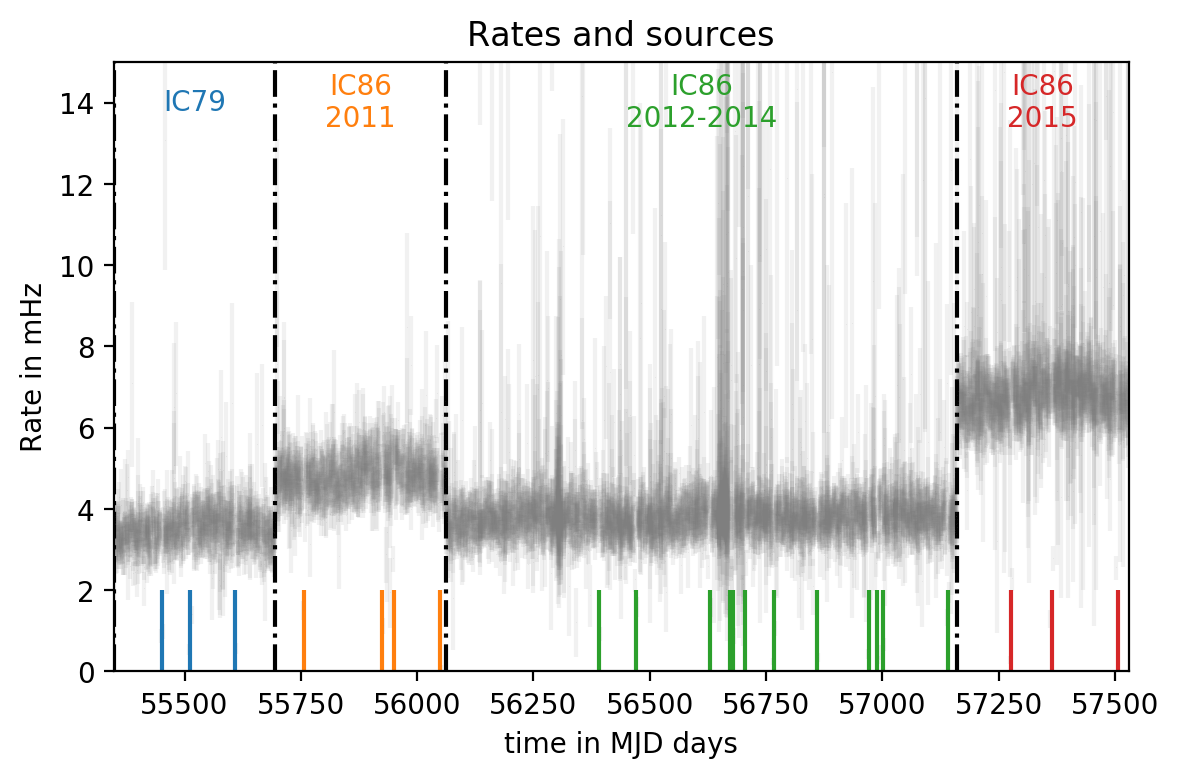
\includegraphics[width=.9\textwidth]{inc/sources_and_rates/rate_all_samples.png}
  \caption{All runs in the off data samples together with the 22 HESE sources per sample. The rates differ per sample due to different event selections. Seasonal variations cause the sinus like variations per year.}
  \label{fig:rate_all_samples}
\end{figure}

\subsubsection{Background Test Statistics}
\begin{figure}[htbp]
  \centering
  \begin{subfigure}[c]{\textwidth}
    \includegraphics[width=0.9\textwidth]{inc/bg_pdfs/bg_pdfs/bg_pdf_tw_00.png}
  \end{subfigure}
  \begin{subfigure}[c]{\textwidth}
    \includegraphics[width=0.9\textwidth]{inc/bg_pdfs/bg_pdfs/bg_pdf_tw_01.png}
  \end{subfigure}
  \begin{subfigure}[c]{\textwidth}
    \includegraphics[width=0.9\textwidth]{inc/bg_pdfs/bg_pdfs/bg_pdf_tw_02.png}
  \end{subfigure}
  \begin{subfigure}[c]{\textwidth}
    \includegraphics[width=0.9\textwidth]{inc/bg_pdfs/bg_pdfs/bg_pdf_tw_03.png}
  \end{subfigure}
  \begin{subfigure}[c]{\textwidth}
    \includegraphics[width=0.9\textwidth]{inc/bg_pdfs/bg_pdfs/bg_pdf_tw_04.png}
  \end{subfigure}
  \begin{subfigure}[c]{\textwidth}
    \includegraphics[width=0.9\textwidth]{inc/bg_pdfs/bg_pdfs/bg_pdf_tw_05.png}
  \end{subfigure}
  \caption{Background trial test statistics for time window 0 to 5. The left subplot show the resulting combined empirical and exponential model. The middle plot the p-value distribution and the right one the p-values for the KS-Test scan.}
\end{figure}

\begin{figure}[htpb]
  \begin{subfigure}[c]{\textwidth}
    \includegraphics[width=0.9\textwidth]{inc/bg_pdfs/bg_pdfs/bg_pdf_tw_06.png}
  \end{subfigure}
  \begin{subfigure}[c]{\textwidth}
    \includegraphics[width=0.9\textwidth]{inc/bg_pdfs/bg_pdfs/bg_pdf_tw_07.png}
  \end{subfigure}
  \begin{subfigure}[c]{\textwidth}
    \includegraphics[width=0.9\textwidth]{inc/bg_pdfs/bg_pdfs/bg_pdf_tw_08.png}
  \end{subfigure}
  \begin{subfigure}[c]{\textwidth}
    \includegraphics[width=0.9\textwidth]{inc/bg_pdfs/bg_pdfs/bg_pdf_tw_09.png}
  \end{subfigure}
  \begin{subfigure}[c]{\textwidth}
    \includegraphics[width=0.9\textwidth]{inc/bg_pdfs/bg_pdfs/bg_pdf_tw_10.png}
  \end{subfigure}
  \caption{Background trial test statistics for time window 6 to 10. The left subplot show the resulting combined empirical and exponential model. The middle plot the p-value distribution and the right one the p-values for the KS-Test scan.}
\end{figure}

\begin{figure}[htpb]
  \begin{subfigure}[c]{\textwidth}
    \includegraphics[width=0.9\textwidth]{inc/bg_pdfs/bg_pdfs/bg_pdf_tw_11.png}
  \end{subfigure}
  \begin{subfigure}[c]{\textwidth}
    \includegraphics[width=0.9\textwidth]{inc/bg_pdfs/bg_pdfs/bg_pdf_tw_12.png}
  \end{subfigure}
  \begin{subfigure}[c]{\textwidth}
    \includegraphics[width=0.9\textwidth]{inc/bg_pdfs/bg_pdfs/bg_pdf_tw_13.png}
  \end{subfigure}
  \begin{subfigure}[c]{\textwidth}
    \includegraphics[width=0.9\textwidth]{inc/bg_pdfs/bg_pdfs/bg_pdf_tw_14.png}
  \end{subfigure}
  \begin{subfigure}[c]{\textwidth}
    \includegraphics[width=0.9\textwidth]{inc/bg_pdfs/bg_pdfs/bg_pdf_tw_15.png}
  \end{subfigure}
  \caption{Background trial test statistics for time window 11 to 15. The left subplot show the resulting combined empirical and exponential model. The middle plot the p-value distribution and the right one the p-values for the KS-Test scan.}
\end{figure}

\begin{figure}[htpb]
  \begin{subfigure}[c]{\textwidth}
    \includegraphics[width=0.9\textwidth]{inc/bg_pdfs/bg_pdfs/bg_pdf_tw_16.png}
  \end{subfigure}
  \begin{subfigure}[c]{\textwidth}
    \includegraphics[width=0.9\textwidth]{inc/bg_pdfs/bg_pdfs/bg_pdf_tw_17.png}
  \end{subfigure}
  \begin{subfigure}[c]{\textwidth}
    \includegraphics[width=0.9\textwidth]{inc/bg_pdfs/bg_pdfs/bg_pdf_tw_18.png}
  \end{subfigure}
  \begin{subfigure}[c]{\textwidth}
    \includegraphics[width=0.9\textwidth]{inc/bg_pdfs/bg_pdfs/bg_pdf_tw_19.png}
  \end{subfigure}
  \begin{subfigure}[c]{\textwidth}
    \includegraphics[width=0.9\textwidth]{inc/bg_pdfs/bg_pdfs/bg_pdf_tw_20.png}
  \end{subfigure}
  \caption{Background trial test statistics for time window 16 to 20. The left subplot show the resulting combined empirical and exponential model. The middle plot the p-value distribution and the right one the p-values for the KS-Test scan.}
\end{figure}

\end{document}